%\documentclass{article}
%\usepackage[utf8]{inputenc}

\documentclass[12pt]{article}
\usepackage{graphicx} % This lets you include figures
\usepackage{hyperref} % This lets you make links to web locations
\graphicspath{ {./images/} }

\usepackage[rightcaption]{sidecap}
\usepackage{subcaption}
\usepackage{wrapfig}

\usepackage{float}

\usepackage{imakeidx}

\makeindex


\title{FEA Visualization Tool}
\author{Thang Nguyen Huu}
\date{\today}

\begin{document}
\maketitle{}

\tableofcontents

\clearpage
\newpage

\section{Application Interface}

%\maketitle{Setup}


\subsection{Load/Open File}

\begin{wrapfigure}{r}{0.50\textwidth} %this figure will be at the right
    \centering
    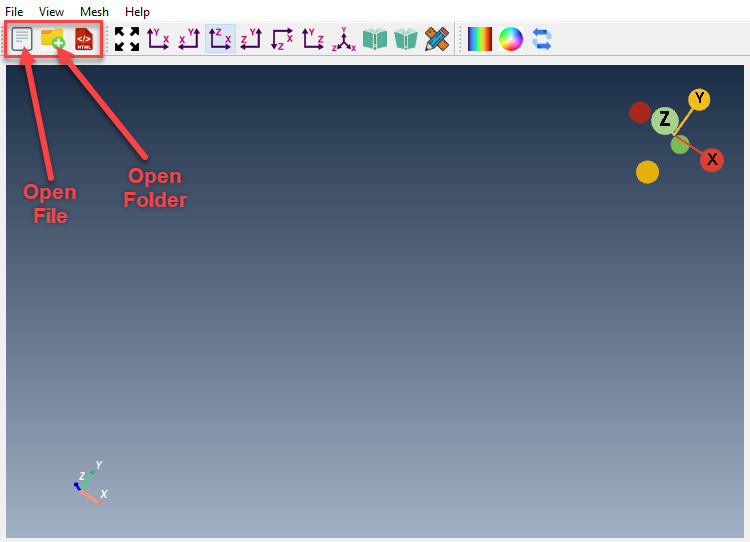
\includegraphics[width=0.50\textwidth]{images/openFile.png}
    \caption{Open data method}
    \label{fig1}
\end{wrapfigure}

You have 2 method to open the data:

- Open by select file.

- Open by select folder.

\ref{fig1} 

If you use the select file method you can open each file in the data folder or view the isolate file.

If you use the select folder method you can open all file with vtk format in the folder.

\vspace{0.2cm}
%\clearpage
\subsection{View Port}

\begin{wrapfigure}{r}{0.5\textwidth}
    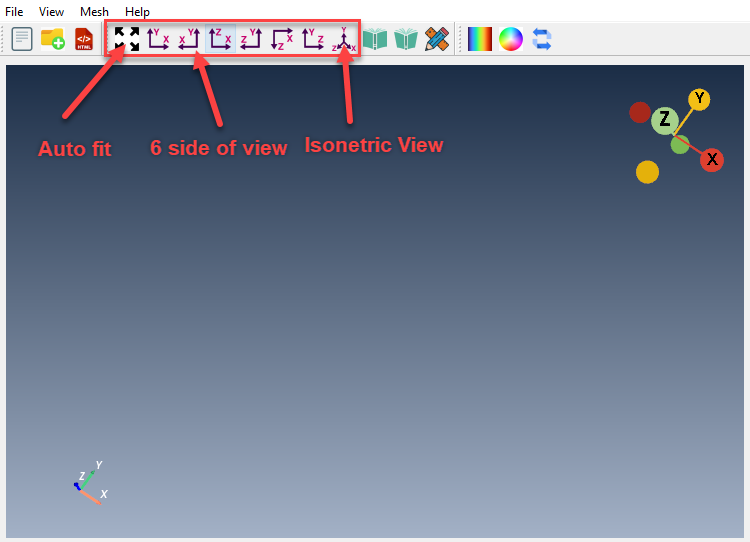
\includegraphics[width=0.5\textwidth]{images/viewPort.png}
    \caption{The Viewport.}
    \label{fig2}
\end{wrapfigure}

You can choose the front, back, left, right, top, bottom and the isometric view by select the corresponding button in the toolbar. \ref{fig2}

If you select the Fit view button, the screen automate view fit all the component.

\newpage

\subsection{View method}

\begin{wrapfigure}{r}{0.5\textwidth}
    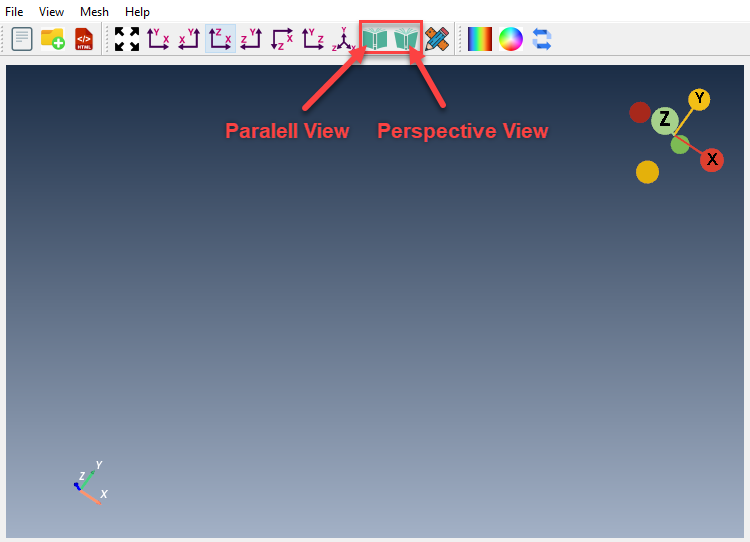
\includegraphics[width=0.5\textwidth]{images/viewMethod.png}
    \caption{View Method.}
    \label{fig3}
\end{wrapfigure}
\vspace{0.2cm}
You can change the view method by select the view parallel or view perspective \ref{fig3}

\subsection{Limit Scalar}
\begin{wrapfigure}{r}{0.5\textwidth}
    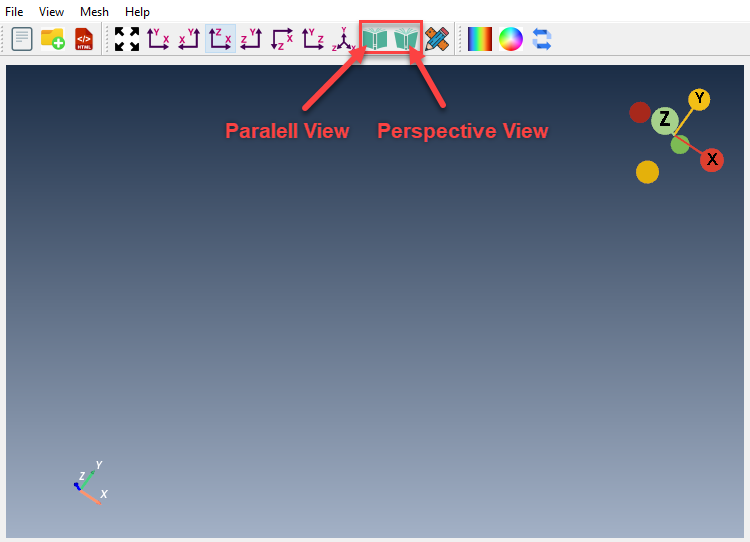
\includegraphics[width=0.5\textwidth]{images/viewMethod.png}
    \caption{Scalar bar limit}
    \label{fig4}
\end{wrapfigure}



You can change limit the scalar bar by enter the input form\ref{fig4}

\clearpage
\newpage

\end{document}
